\documentclass[11pt]{article}
\usepackage[a4paper,margin=0.86in]{geometry}
\usepackage{amsmath,amssymb,amsthm,mathtools}
\usepackage{booktabs,array}
\usepackage{graphicx}
\usepackage{xcolor}
\usepackage[hidelinks]{hyperref}
\hypersetup{
  pdftitle={Complete Delay--Memory Regions for Passive Quantum Networks},
  pdfauthor={Lluis Eriksson},
  pdfsubject={Majorization synthesis, rational quantization, and Pick memory tomography}
}
\usepackage[nameinlink,capitalise]{cleveref}
\usepackage{microtype}

\newtheorem{theorem}{Theorem}[section]
\newtheorem{proposition}[theorem]{Proposition}
\newtheorem{lemma}[theorem]{Lemma}
\newtheorem{corollary}[theorem]{Corollary}
\theoremstyle{definition}
\newtheorem{definition}[theorem]{Definition}
\newtheorem{example}[theorem]{Example}
\theoremstyle{remark}
\newtheorem{remark}[theorem]{Remark}
\newtheorem{limitation}[theorem]{Limitation}

\newcommand{\C}{\mathbb C}
\newcommand{\D}{\mathbb D}
\newcommand{\T}{\mathbb T}
\newcommand{\tr}{\operatorname{tr}}
\newcommand{\rank}{\operatorname{rank}}
\newcommand{\ran}{\operatorname{ran}}
\newcommand{\diag}{\operatorname{diag}}
\newcommand{\dd}{\mathrm d}
\newcommand{\e}{\mathrm e}
\newcommand{\mcdeg}{\deg_{\mathrm{McM}}}
\newcommand{\opnorm}[1]{\lVert#1\rVert_{\mathrm{op}}}
\newcommand{\pos}[1]{\left[#1\right]_{+}}

\title{Complete Delay--Memory Regions for Passive Quantum Networks:\\
Majorization Synthesis, Rational Quantization, and Pick Tomography}
\author{Lluis Eriksson}
\date{10 August 2026}

\begin{document}
\maketitle

\begin{abstract}
Lower bounds do not determine which resource profiles are physically
attainable.  We close that inverse problem for passive subspace transport.
Let two rank-$k$ subspaces in $\C^N$, $N\geq2k$, have ordered canonical
angles $\beta$, and let
$q_j=\int\lambda_j(Q(t))\,\dd t$ be the integrated leading eigenvalues of a
positive generator $Q=-\mathrm iS^*\dot S$.  We prove the exact equivalence
\[
 q\text{ is attainable}\quad\Longleftrightarrow\quad 2\beta\prec_w q.
\]
Every feasible profile has a compiler using at most $k+1$ mutually commuting,
positive generators of rank at most $k$ whose ordered top spectrum is constant
in time;
the Carath\'eodory count is generically sharp within this signed-orbit
compiler class.  Analytic rationality adds a
different, integer-valued resource.  For two boundary frequencies, the least
McMillan degree of an inner matrix that sends a fixed input subspace to two
prescribed output subspaces is exactly the number of nonzero canonical
angles.  Thus arbitrarily small full-rank motion has vanishing continuous
action but a fixed $k$-state memory cost.  We give a fail-closed finite-error
certificate for both resources from noisy projectors.

At multiple frequencies, we show that Wigner--Smith delay is only the
block diagonal of a boundary de Branges--Rovnyak Pick matrix.  This matrix is
positive, has rank at most the McMillan degree, and is the Gram matrix of the
internal states excited by the measured frequencies and channels.  Its
spectrum yields robust degree certificates and unavoidable model-reduction
tails.  An exact scalar example has identical proper delays at two frequencies
for degree one and degree two, while the corresponding Pick ranks are one and
two.  A transfer-matrix corollary identifies Euclidean correlators as Fourier
coefficients of a proper-delay spectrum and a spectral gap as a zero-frequency
delay cap; it is a dictionary, not a mass-gap proof.  Deterministic code
reconstructs the compilers, tests $2{,}240$ randomized theorem interfaces,
checks the strict separation, and independently replays the certificate.
\end{abstract}

\noindent\textbf{Keywords:} passive quantum network; Wigner--Smith delay;
weak majorization; McMillan degree; rational inner function; Pick matrix;
de Branges--Rovnyak kernel; subspace transport; mass gap.

\section{Two resources hidden in one routing event}

The preceding papers in this programme progressed from finite-sample
spectral exclusion and noncommuting architectural separation to passive
reservoir filters, topological memory, robust routing and a complete Ky Fan
speed-limit hierarchy
\cite{ErikssonFinite2026,ErikssonMIMO2026,ErikssonReservoir2026,
ErikssonMemory2026,ErikssonRouting2026,ErikssonKyFan2026}.
The sixth paper proved that if a rank-$k$ subspace moves through canonical
angles $\beta_1\geq\cdots\geq\beta_k$, then its integrated proper-delay
profile $q$ must satisfy
\begin{equation}\label{eq:necessary}
 2\beta\prec_w q,
 \qquad
 2\sum_{j=1}^r\beta_j\leq\sum_{j=1}^r q_j,
 \quad r=1,\ldots,k.
\end{equation}
Every symmetric-gauge minimum follows from this Lorenz-curve inequality.
What remained open was whether \eqref{eq:necessary} is merely an obstruction
or the complete feasible region.

We answer that question and then expose a second resource that no continuous
speed limit can see.  A rational inner transfer matrix has an integer
McMillan degree.  We prove that the least degree needed to create a two-point
subspace rotation is the support size of the canonical-angle vector, not its
norm.  Continuous action prices the amplitude of motion; rational degree
prices how many independent directions move at all.

The multi-frequency completion is a positive kernel.  For a rational inner
$S$ define
\begin{equation}\label{eq:kernelintro}
 K_S(z,w)=\frac{I-S(z)S(w)^*}{1-z\bar w}.
\end{equation}
At a boundary point its diagonal is a unitary conjugate of Wigner--Smith
delay.  Off the diagonal it records overlaps between frequency-excited
internal states.  Those cross terms distinguish devices whose local delay
spectra agree.

The ingredients are classical and we keep the priority boundary explicit.
Weak majorization and signed permutahedra belong to majorization theory
\cite{MarshallOlkinArnold2011}; Grassmann metrics are due to Qiu, Zhang and
Li \cite{QiuZhangLi2005}, with a recent projector-based treatment of shortest
Grassmann paths given by Huang \cite{Huang2026}; spectral-spread block inequalities are due to
Massey, Stojanoff and Z\'arate \cite{MasseyStojanoffZarate2021}; boundary
Schur interpolation and de Branges--Rovnyak spaces are established theories
\cite{deBrangesRovnyak1966,BolotnikovDym2006}; and minimal passive quantum
realizations are classical system theory
\cite{McMillan1952,GoughZhang2015}.  Our contribution is the exact attainable
delay region and compiler, the sharp two-subspace degree quantization, their
joint robust certificate, and the operational Pick--Wigner--Smith memory
tomography built from finite scattering data.

\section{Setup and the necessary Lorenz law}

Let $\mathcal X,\mathcal Y\subset\C^N$ have rank $k$, with $N\geq2k$.
Their ordered canonical angles are
$\beta_1\geq\cdots\geq\beta_k\in[0,\pi/2]$.
Let $S:[0,\Delta]\to U(N)$ be absolutely continuous,
$S(0)\mathcal X=\mathcal X$ and $S(\Delta)\mathcal X=\mathcal Y$, and put
\begin{equation}\label{eq:generator}
 Q(t)=-\mathrm iS(t)^*\dot S(t).
\end{equation}
We call the path passive-monotone when $Q(t)\succeq0$ almost everywhere.
Its integrated leading-delay profile is
\begin{equation}\label{eq:qprofile}
 q_j=\int_0^\Delta\lambda_j(Q(t))\,\dd t,
 \qquad q_1\geq\cdots\geq q_k\geq0.
\end{equation}

The time-dependent spectral-spread theorem of
\cite{ErikssonKyFan2026}, obtained by composing a Grassmann path-length law
with the block inequality of \cite{MasseyStojanoffZarate2021}, gives
\eqref{eq:necessary}.  This is the only necessity input used below.

\section{The complete delay region}

Write $\mathfrak B_k$ for the group of signed permutation matrices.  A
standard orbit-polytope form of weak majorization says, for nonnegative
decreasing $x,q\in\mathbb R^k$,
\begin{equation}\label{eq:signedpolytope}
 x\prec_wq
 \quad\Longleftrightarrow\quad
 x\in\operatorname{conv}\{Rq:R\in\mathfrak B_k\}.
\end{equation}
The signs, which are irrelevant to symmetric norms, acquire a physical
meaning here: they reverse motion in a principal plane while preserving
positive proper delay.

\begin{theorem}[Complete positive-delay region]\label{thm:complete}
Let $N\geq2k$ and let $q\in\mathbb R^k$ be nonnegative and decreasing.
There exists an absolutely continuous path transporting $\mathcal X$ to
$\mathcal Y$, with $Q(t)\succeq0$ and integrated profile \eqref{eq:qprofile},
if and only if
\begin{equation}\label{eq:completecondition}
 2\beta\prec_wq.
\end{equation}
Whenever \eqref{eq:completecondition} holds, there is such a path with all of
the following properties:
\begin{enumerate}
 \item at most $k+1$ piecewise-constant segments;
 \item $\rank Q(t)\leq k$;
 \item $(\lambda_1(Q(t)),\ldots,\lambda_k(Q(t)))=q/\Delta$ almost everywhere;
 \item all segment generators commute.
\end{enumerate}
The same equivalence holds if $q$ denotes the integrated first $k$ spectral
spreads of an arbitrary Hermitian generator.
\end{theorem}

\begin{proof}
Necessity is \eqref{eq:necessary}.  For sufficiency, apply
\eqref{eq:signedpolytope} and Carath\'eodory's theorem in $\mathbb R^k$:
there are $m\leq k+1$, weights $t_s\geq0$ summing to one and
$R_s\in\mathfrak B_k$ such that
\begin{equation}\label{eq:barycenter}
 2\beta=\sum_{s=1}^m t_sR_sq.
\end{equation}
Choose principal pairs $e_j,f_j$ so that
\[
 \mathcal X=\operatorname{span}\{e_j\}_{j=1}^k,
 \qquad
 \mathcal Y=\operatorname{span}\{\cos\beta_j e_j-\sin\beta_j f_j\}_{j=1}^k.
\]
Write $(R_sq)_j=\varepsilon_{s,j}q_{\pi_s(j)}$.
On a segment of duration $t_s\Delta$, define, in the plane
$\operatorname{span}\{e_j,f_j\}$,
\begin{equation}\label{eq:compilerblock}
 Q_{s,j}=\frac{q_{\pi_s(j)}}{2\Delta}
 \begin{bmatrix}1&-\mathrm i\varepsilon_{s,j}\\
 \mathrm i\varepsilon_{s,j}&1\end{bmatrix}.
\end{equation}
Each block is positive with eigenvalues $q_{\pi_s(j)}/\Delta$ and zero.
Thus $Q_s=\bigoplus_jQ_{s,j}$ has rank at most $k$ and ordered top spectrum
$q/\Delta$.

For a fixed plane, the two possible normalized blocks in
\eqref{eq:compilerblock} are complementary rank-one projections, so they
commute; blocks in distinct planes also commute.  The signed rotation
accumulated in plane $j$ is
\[
 \frac12\sum_s t_s\varepsilon_{s,j}q_{\pi_s(j)}=\beta_j
\]
by \eqref{eq:barycenter}.  Hence the endpoint is $\mathcal Y$ and the
integrated ordered spectrum is exactly $q$.  The constructed positive
rank-$k$ generator has $N-k$ zero eigenvalues, so its first $k$ spectral
spreads also equal its leading eigenvalues.  Unitary conjugation places the
construction in arbitrary principal frames.
\end{proof}

\begin{proposition}[Sharpness within signed-orbit compilation]\label{prop:segments}
If $q_1>\cdots>q_k>0$, then almost every point in the signed permutahedron
$\operatorname{conv}(\mathfrak B_kq)$ requires $k+1$ vertices in a convex
representation.  Consequently, the $k+1$ segment count in the signed-orbit
construction of \cref{thm:complete} cannot be lowered uniformly within that
compiler class.
\end{proposition}

\begin{proof}
The signed permutahedron is full-dimensional.  The points representable by at
most $k$ vertices form a finite union of simplices of dimension at most
$k-1$, hence have Lebesgue measure zero.
\end{proof}

This is not a lower bound for unrestricted constant positive generators.
Already for $k=1$, tilting the eigenvector of one rank-one generator can
realize some interior angles with a single segment even when the signed-orbit
decomposition uses two.  Proposition~\ref{prop:segments} concerns the explicit
block-efficient compiler only.

The theorem gives the complete spectrum between two familiar extremes.
$q=2\beta$ is the Pareto frontier and moves all principal planes in parallel.
The profile
\begin{equation}\label{eq:serial}
 q=(2\sum_j\beta_j,0,\ldots,0)
\end{equation}
serializes every rotation through one instantaneous delay mode.  All profiles
above the Lorenz frontier interpolate exactly between parallel and serial
architectures; there are no hidden continuous inequalities.

\section{Rational quantization: support costs memory}

The continuous theorem allows arbitrarily small nonzero angles at arbitrarily
small action.  A rational inner device obeys an additional integer law.
Let $\zeta_0\ne\zeta_1\in\T$ and let $S$ be an $N\times N$ rational inner
matrix regular at both nodes.  For a fixed rank-$k$ input subspace
$\mathcal X$, put $\mathcal Y_i=S(\zeta_i)\mathcal X$ and let $\beta$ be the
canonical-angle vector between $\mathcal Y_0$ and $\mathcal Y_1$.

\begin{theorem}[Exact two-frequency memory quantization]\label{thm:quantization}
Let
\begin{equation}\label{eq:rbeta}
 r_\beta=\#\{j:\beta_j>0\}
 =k-\dim(\mathcal Y_0\cap\mathcal Y_1).
\end{equation}
Then
\begin{equation}\label{eq:minimaldegree}
 \boxed{\qquad
 \min_S\mcdeg(S)=r_\beta,
 \qquad}
\end{equation}
where the minimum is over rational inner matrices satisfying the two
subspace constraints at fixed external dimension $N$.  Moreover, the
minimizing construction can obey
\begin{equation}\label{eq:localactionsaturation}
 \int_I\tr Q(\theta)\,\dd\theta=2\sum_{j=1}^k\beta_j
\end{equation}
on the positively oriented arc $I$ from $\zeta_0$ to $\zeta_1$ (either
geometric arc may be selected by ordering the two nodes accordingly).
\end{theorem}

\begin{proof}
Let $n=\mcdeg(S)$ and use a minimal realization
\[
 S(z)=D+zC(I-zA)^{-1}B,
 \qquad A\in\C^{n\times n}.
\]
The resolvent identity gives
\begin{equation}\label{eq:rankdifference}
 S(z)-S(w)=(z-w)C(I-zA)^{-1}(I-wA)^{-1}B,
\end{equation}
so $\rank(S(z)-S(w))\leq n$.  The kernel of
$(S(\zeta_1)-S(\zeta_0))|_{\mathcal X}$ has dimension at least $k-n$, and
every vector in that kernel has a common image in
$\mathcal Y_0\cap\mathcal Y_1$.  Hence $r_\beta\leq n$.

For the converse, choose principal planes for the nonzero angles.  A disk
automorphism $b_j$ can be chosen with
\begin{equation}\label{eq:boundaryphase}
 b_j(\zeta_0)=1,
 \qquad b_j(\zeta_1)=\e^{2\mathrm i\beta_j};
\end{equation}
this is the two-point transitivity of disk automorphisms on the boundary.
With $H_2=2^{-1/2}\bigl[\begin{smallmatrix}1&1\\1&-1\end{smallmatrix}\bigr]$,
the degree-one inner block
\begin{equation}\label{eq:interferometer}
 R_j(z)=H_2\diag(1,b_j(z))H_2
\end{equation}
is the identity at $\zeta_0$ and sends the first coordinate line at
$\zeta_1$ through angle $\beta_j$.  Constant unitaries align the resulting
planes with the prescribed principal vectors.  The direct sum of the
$r_\beta$ nonconstant blocks and constant identity blocks has degree
$r_\beta$.

The boundary phase of a Blaschke factor is strictly increasing.  Choose the
automorphism in \eqref{eq:boundaryphase} so that its unwrapped phase advance
on $I$ is $2\beta_j$.  The trace of the Wigner--Smith matrix of
\eqref{eq:interferometer} is precisely that phase derivative.  Summing the
blocks proves \eqref{eq:localactionsaturation}.
\end{proof}

\begin{corollary}[Topological complementarity]\label{cor:complementarity}
Every degree-minimal construction in the proof stores
\begin{equation}\label{eq:outsidephase}
 2\pi r_\beta-2\sum_j\beta_j
\end{equation}
of its total trace action outside the selected arc.  In particular, if
$\beta_j=\varepsilon>0$ for all $j$, then
\begin{equation}\label{eq:vanishingaction}
 \mcdeg(S)\geq k
 \quad\text{while}\quad
 \inf\int_I\tr Q=2k\varepsilon\longrightarrow0.
\end{equation}
\end{corollary}

This is the sharp separation between amplitude and support.  The continuous
Lorenz region has no discontinuity at zero, whereas rational memory jumps by
one whenever a new canonical direction becomes nontrivial.

\section{One noisy measurement certifies both resources}

Let $P_i$ be the projections onto $\mathcal Y_i$ and suppose tomography gives
rank-$k$ orthogonal projections $\widehat P_i$ with
\begin{equation}\label{eq:projectorerror}
 \opnorm{\widehat P_i-P_i}\leq\eta_i.
\end{equation}
Let $\widehat s_1\geq\cdots\geq\widehat s_k$ be the $k$ largest singular
values of $(I-\widehat P_0)\widehat P_1$.

\begin{theorem}[Fail-closed joint certificate]\label{thm:robustprojector}
With $\eta=\eta_0+\eta_1$, define
\begin{equation}\label{eq:certangles}
 \beta_j^{\rm cert}=\arcsin\!\left(\min\{1,\pos{\widehat s_j-\eta}\}\right).
\end{equation}
Then, on the event \eqref{eq:projectorerror}, every square rational inner
$S$ regular at the two nodes and realizing the subspace data obeys
\begin{align}
 \mcdeg(S)&\geq\#\{j:\widehat s_j>\eta\},\label{eq:robustdegree}\\
 \int_I\sum_{j=1}^r\lambda_j(Q)\,\dd\theta
 &\geq2\sum_{j=1}^r\beta_j^{\rm cert},
 \qquad r=1,\ldots,k.\label{eq:robustlorenz}
\end{align}
Values exactly at the threshold are never counted.
\end{theorem}

\begin{proof}
Writing $A=(I-P_0)P_1$ and
$\widehat A=(I-\widehat P_0)\widehat P_1$ gives
$\opnorm{A-\widehat A}\leq\eta_0+\eta_1$.  The nonzero singular values of
$A$ are $\sin\beta_j$.  Weyl's singular-value inequality proves
$\sin\beta_j\geq\pos{\widehat s_j-\eta}$.  Apply
\cref{thm:quantization} for \eqref{eq:robustdegree} and the positive-delay
hierarchy on the positively oriented arc $I$ for \eqref{eq:robustlorenz}.
\end{proof}

The output is simultaneously discrete and continuous: a certified number of
internal states and a certified lower Lorenz curve for the action those states
must carry.

\section{Proper delays are diagonal memory}

The two-frequency theorem counts directions that move.  More sampling points
can reveal hidden state directions that no single pair or collection of local
delay spectra resolves.  Let $S:\D\to\C^{p\times p}$ be rational inner of
degree $d$, regular at distinct boundary nodes
$\zeta_1,\ldots,\zeta_L$.  Put
\begin{equation}\label{eq:boundarydata}
 U_i=S(\zeta_i),
 \qquad
 Q_i=-\mathrm iU_i^*\partial_\theta S(\e^{\mathrm i\theta})|_{\zeta_i}.
\end{equation}
Define the $Lp\times Lp$ block matrix
\begin{equation}\label{eq:pickgram}
 G_{ij}=\begin{cases}
 \displaystyle\frac{I-U_iU_j^*}{1-\zeta_i\bar\zeta_j},&i\ne j,\\[1.2ex]
 U_iQ_iU_i^*,&i=j.
 \end{cases}
\end{equation}

\begin{theorem}[Pick--Wigner--Smith memory theorem]\label{thm:pick}
The finite-data matrix \eqref{eq:pickgram} satisfies
\begin{equation}\label{eq:pickrank}
 G\succeq0,
 \qquad
 \rank G\leq d.
\end{equation}
For a minimal unitary realization there are matrices
$F_i\in\C^{p\times d}$ such that
\begin{equation}\label{eq:gramfactor}
 G_{ij}=F_iF_j^*.
\end{equation}
Thus $G$ is the Gram matrix of the internal states excited by the sampled
frequencies and channels.  Equality $\rank G=d$ holds exactly when those
states span the realization space.
\end{theorem}

\begin{proof}
Every square rational inner function admits a minimal conservative unitary
colligation whose state dimension is $d=\mcdeg(S)$; regularity at the sampled
boundary nodes ensures the boundary resolvents below exist.  Take such a
realization
\[
 S(z)=D+zC(I-zA)^{-1}B.
\]
The lossless realization identity is
\begin{equation}\label{eq:kernelidentity}
 \frac{I-S(z)S(w)^*}{1-z\bar w}
 =C(I-zA)^{-1}(I-\bar wA^*)^{-1}C^*.
\end{equation}
Set $F_i=C(I-\zeta_iA)^{-1}$.  Off the diagonal,
\eqref{eq:gramfactor} follows directly.  On the boundary diagonal, the
Carath\'eodory--Julia limit gives
\begin{equation}\label{eq:diagonalidentity}
 K_S(\zeta_i,\zeta_i)
 =\zeta_iS'(\zeta_i)U_i^*=U_iQ_iU_i^*,
\end{equation}
which proves the same factorization.  Positivity and the rank bound are now
immediate.
\end{proof}

The pinching inequality gives a spectral statement that local delays alone
cannot reverse:
\begin{equation}\label{eq:pinching}
 \lambda\!\left(\bigoplus_iU_iQ_iU_i^*\right)
 \prec\lambda(G).
\end{equation}
Cross-frequency coherence can concentrate many nonzero local delay blocks in
a much smaller hidden state space.  Two convenient degree lower bounds are
\begin{equation}\label{eq:effectiverank}
 d\geq\rank G
 \geq\frac{(\tr G)^2}{\tr(G^2)}.
\end{equation}

\begin{example}[Equal local delays, different hidden memory]\label{ex:blindness}
Take scalar nodes $\zeta_1=1$, $\zeta_2=-1$ and
\begin{equation}\label{eq:blindfunctions}
 S_1(z)=z,
 \qquad
 S_2(z)=\left(\frac{z-\mathrm i/\sqrt3}{1+\mathrm iz/\sqrt3}\right)^2.
\end{equation}
The scalar proper delay of a Blaschke product is the sum of its Poisson
kernels.  Direct substitution gives
\begin{equation}\label{eq:samedelays}
 Q_1(1)=Q_1(-1)=Q_2(1)=Q_2(-1)=1.
\end{equation}
Nevertheless,
\begin{equation}\label{eq:strictpick}
 \lambda(G_1)=(2,0),
 \qquad
 \lambda(G_2)=(1+\sqrt3/2,1-\sqrt3/2).
\end{equation}
Thus the two local delay lists are identical, while the Pick ranks recover
degrees one and two exactly.  The missing information is entirely in the
measured scattering phases and hence in the off-diagonal blocks.
\end{example}

\section{Robust Pick rank and reduction barriers}

Suppose $\widehat U_i$ are unitary estimates and $\widehat Q_i$ are Hermitian
estimates satisfying
\begin{equation}\label{eq:pickerrors}
 \max_i\opnorm{\widehat U_i-U_i}\leq\varepsilon_U,
 \qquad
 \max_i\opnorm{\widehat Q_i-Q_i}\leq\varepsilon_Q,
 \qquad
 \max_i\opnorm{Q_i}\leq q_{\max}.
\end{equation}
Let
\begin{equation}\label{eq:nodeseparation}
 \delta=\min_{i\ne j}|1-\zeta_i\bar\zeta_j|>0
\end{equation}
and build $\widehat G$ from the measured data by \eqref{eq:pickgram}.

\begin{theorem}[Deterministic noisy-memory certificate]\label{thm:robustpick}
Define
\begin{equation}\label{eq:eta}
 \eta_G=\varepsilon_Q+2q_{\max}\varepsilon_U
 +(L-1)\frac{2\varepsilon_U}{\delta}.
\end{equation}
Then $\opnorm{\widehat G-G}\leq\eta_G$ and therefore
\begin{equation}\label{eq:rankthreshold}
 \boxed{\qquad
 d\geq\#\{j:\lambda_j(\widehat G)>\eta_G\}.
 \qquad}
\end{equation}
If $\lambda_{\min}(\widehat G)<-\eta_G$, no rational inner network is
compatible with the stated error budget.
\end{theorem}

\begin{proof}
For diagonal blocks, unitary invariance and \eqref{eq:pickerrors} give
\[
 \opnorm{\widehat U_i\widehat Q_i\widehat U_i^*-U_iQ_iU_i^*}
 \leq\varepsilon_Q+2q_{\max}\varepsilon_U.
\]
For $i\ne j$, the corresponding bound is
$2\varepsilon_U/|1-\zeta_i\bar\zeta_j|$.
The block row-sum bound proves \eqref{eq:eta}; Weyl's theorem and
\cref{thm:pick} prove \eqref{eq:rankthreshold} and the falsifier.
\end{proof}

\begin{corollary}[Unavoidable reduction tails]\label{cor:reduction}
Let $G$ be the exact memory Gram matrix of a device.  Every degree-$r$
rational inner approximant, with corresponding sample matrix $\widetilde G$,
satisfies
\begin{align}
 \opnorm{G-\widetilde G}&\geq\lambda_{r+1}(G),\label{eq:opertail}\\
 \lVert G-\widetilde G\rVert_F
 &\geq\left(\sum_{j>r}\lambda_j(G)^2\right)^{1/2}.
 \label{eq:frobtail}
\end{align}
More generally, every unitarily invariant norm is bounded below by the
matching spectral tail.
\end{corollary}

\begin{proof}
$\rank\widetilde G\leq r$ by \cref{thm:pick}; apply the
Eckart--Young--Mirsky theorem.
\end{proof}

This is a model-reduction obstruction in measured coordinates, not an
asymptotic statement about a chosen identification algorithm.

\section{A transfer-matrix corollary}

The positive-kernel viewpoint also gives a precise bridge to transfer
matrices.  Let $0<T<I$ be a finite-dimensional positive self-adjoint
contraction and define
\begin{equation}\label{eq:transferinner}
 S_T(z)=(zI-T)(I-zT)^{-1}.
\end{equation}
This self-adjoint Schur-to-inner transform is classical
\cite{ArlinskiiHassi2018}; we record its consequence for delay and Euclidean
correlators.

\begin{proposition}[Transfer--delay dictionary]\label{prop:dictionary}
The function \eqref{eq:transferinner} is inner and
\begin{align}
 Q_T(\theta)
 &=\bigl(I-T^2\bigr)
 \bigl(I-2T\cos\theta+T^2\bigr)^{-1},\label{eq:poisson}\\
 &=I+2\sum_{n\geq1}T^n\cos(n\theta).\label{eq:fourier}
\end{align}
Hence, for any observable map $V$, the Euclidean correlators
$C_n=V^*T^nV$ are exactly the complex Fourier coefficients of
$V^*Q_T(\theta)V$ (equivalently, the coefficients in its cosine expansion
\eqref{eq:fourier}).  If $T=\e^{-H}$ on a vacuum-orthogonal sector, then
\begin{equation}\label{eq:massdelay}
 Q_T(0)=\coth(H/2),
 \qquad
 H\succeq mI
 \Longleftrightarrow
 Q_T(0)\preceq\coth(m/2)I.
\end{equation}
\end{proposition}

\begin{proof}
Diagonalize $T$ and apply the scalar Blaschke and Poisson-kernel identities to
each eigenvalue.  Equation \eqref{eq:massdelay} follows by functional calculus
and monotonicity of $t\mapsto(1+t)/(1-t)$.
\end{proof}

For the $SU(2)$ heat semigroup used in two-dimensional Yang--Mills, the
non-vacuum class-function eigenvalues are
$\exp[-a n(n+2)/4]$, $n\geq1$.  Therefore
\begin{equation}\label{eq:su2}
 h_n=\frac{a n(n+2)}4,
 \qquad
 q_n(0)=\coth\!\left(\frac{a n(n+2)}8\right),
 \qquad
 \opnorm{Q(0)}=\coth(3a/8).
\end{equation}
The semigroup and its $SU(2)$ spectrum are independently formalized in the
companion Lean development \cite{ErikssonLeanYM2026}.

\begin{limitation}[Dictionary, not a mass-gap proof]
Equation \eqref{eq:massdelay} reparametrizes a known transfer spectrum; it
does not establish a gap for an interacting theory.  The vacuum eigenvalue
$T=1$ must be projected out.  A compression $V^*Q_TV$ sees only the cyclic
sector generated by $V$ and can miss a slower orthogonal mode exactly.
Infinite-dimensional field theories also lie outside the rational
finite-degree statements of \cref{thm:quantization,thm:pick}.
\end{limitation}

This restricted corollary is included because it gives a falsifiable bridge
between the passive-network resource and Euclidean data without claiming a
solution of the Yang--Mills mass-gap problem.

\section{Reproducible adversarial audit}

All principal results are analytic.  The computational artifact attacks the
constructive and finite-precision interfaces:
\begin{enumerate}
 \item a flagship rank-three profile with four compiler segments, positive
 Lorenz margins, endpoint error $4.5\times10^{-16}$ and commutator norm below
 $10^{-16}$;
 \item $192$ random feasible profiles of ranks one through four, each solved
 by linear programming over its signed permutahedron and reconstructed by
 exact matrix exponentials; the worst endpoint/profile error is below
 $4.5\times10^{-14}$ and no compiler uses more than $k+1$ segments;
 \item $256$ random two-node Blaschke compilers, verifying endpoint phases,
 principal angles, positive delay and the sharp integrated arc action;
 \item $512$ noisy rank-$k$ projector pairs, with no degree overcount and no
 violation of any certified Lorenz prefix;
 \item the exact degree-one/degree-two blindness example
 \eqref{eq:blindfunctions}--\eqref{eq:strictpick};
 \item $768$ random matrix Blaschke--Potapov networks, with no Pick-rank
 violation and $743$ generic full-degree recoveries;
 \item $512$ noisy matrix instances, with no robust rank overcount and a
 largest actual-error/bound ratio below $0.476$; and
 \item the transfer identity on $8{,}192$ Fourier nodes, recovering four
 coefficients with error below $2.6\times10^{-15}$.
\end{enumerate}
An independent verifier rebuilds the compiler from the frozen signed vertices,
checks positivity, commutativity, endpoint angles and exact delay profile,
rederives the strict example, and runs separately coded scalar and matrix Pick,
noisy-projector, noisy-rank and Blaschke-action probes.  The JSON certificate,
figure, source and release manifest are hash-locked and replayed in continuous
integration.

\begin{figure}[t]
 \centering
 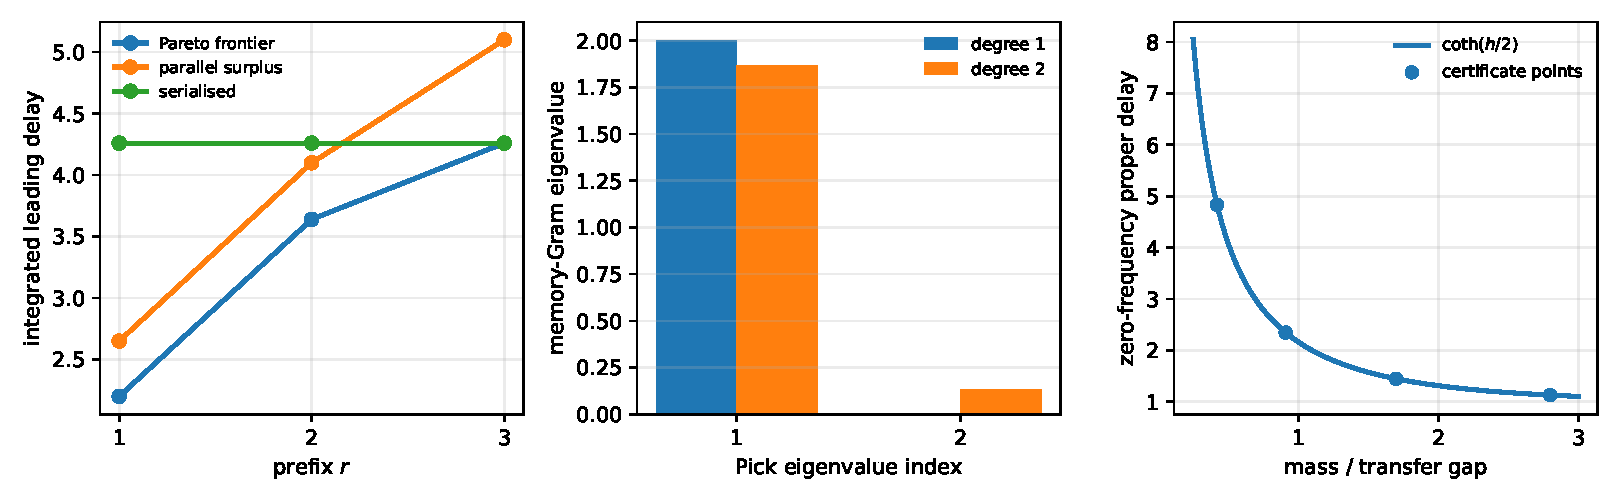
\includegraphics[width=\linewidth]{figures/complete_region.pdf}
 \caption{Left: the complete Lorenz region contains parallel, surplus and
 serial resource allocations.  Centre: two scalar networks have identical
 local proper delays at both nodes, but Pick spectra of ranks one and two.
 Right: the transfer gap and zero-frequency delay are related exactly by
 $q=\coth(h/2)$.}
 \label{fig:summary}
\end{figure}

\section{Scope, falsifiers and open problems}

\begin{limitation}[Continuous synthesis is not rational synthesis]
The compiler in \cref{thm:complete} is an absolutely continuous unitary path
with piecewise-constant positive generator.  It need not be the boundary trace
of a rational inner function of a prescribed degree.  The quantization theorem
solves exactly the two-node subspace problem, not arbitrary profile
interpolation on a whole arc.
\end{limitation}

\begin{limitation}[Subspaces, not calibrated frames]
The degree $r_\beta$ is exact for subspace constraints.  Prescribing phases or
complete frames can require additional degree.  Conversely, allowing hidden
loss ports requires a unitary dilation before any inner or Wigner--Smith rank
claim is applied.
\end{limitation}

\begin{limitation}[Node separation is a resource]
The robust Pick threshold deteriorates as
$\delta=\min_{i\ne j}|1-\zeta_i\bar\zeta_j|$ tends to zero.  Closely spaced
samples require derivative data of higher accuracy or a confluent Pick
formulation.  A substantially negative eigenvalue beyond \eqref{eq:eta}
falsifies the claimed lossless passive model.
\end{limitation}

Three questions now have precise targets: characterize the rational-inner
subset of the full Lorenz region at fixed degree; derive a confluent robust
kernel for clustered frequency samples; and determine when small Pick tails
imply an operator-norm-nearby passive reduced model, rather than only the
necessary lower bounds \eqref{eq:opertail}--\eqref{eq:frobtail}.

\section{Conclusion}

Passive subspace transport has a complete continuous resource region:
$2\beta\prec_wq$ is necessary and sufficient, and every feasible point is
compiled by at most $k+1$ commuting positive segments with constant proper-delay
spectrum.  Rationality then quantizes a transverse resource: the minimum
memory degree is the number of nonzero canonical angles.  One noisy projector
spectrum certifies both the integer support cost and the continuous Lorenz
cost.

Across multiple frequencies, proper delays are only diagonal memory.  The
boundary Pick matrix restores the missing cross-frequency coherences, is
literally a Gram matrix of internal states, and yields robust rank and
model-reduction obstructions.  The strict degree-one/degree-two example proves
that this information is operationally new.  The resulting picture is a
two-layer resource theory: majorization controls how much motion is required,
while analytic rank controls how many hidden states must exist to realize it.

\section*{Data and code availability}

The final manuscript, generator, independent verifier, frozen JSON
certificate, figure and hash manifest are archived in the immutable
\href{https://github.com/lluiseriksson/finite-sample-spectral-certificates/releases/tag/v1.6-complete-delay-memory-regions}{GitHub release v1.6}
of the companion repository.
Theorems are proved analytically in the text; numerical tests are adversarial
audits and do not substitute for the proofs.

\bibliographystyle{plain}
\bibliography{references}

\end{document}
